% ═══════════════════════════════════════════════════════════════
%  Weekly Meeting – 24 April 2026
%  Full-Database Heterogeneity Validation
%  Sphere Region Method, Pflugfelder HI & WEPL
%  Author: Mikołaj Stryja
% ═══════════════════════════════════════════════════════════════
\documentclass[aspectratio=169, 10pt]{beamer}

% ── Theme & colours ─────────────────────────────────────────
\usetheme{Madrid}
\usecolortheme{default}
\definecolor{tudelft}{RGB}{0,100,172}
\setbeamercolor{structure}{fg=tudelft}
\setbeamercolor{title}{fg=white,bg=tudelft}
\setbeamercolor{frametitle}{fg=white,bg=tudelft}
\setbeamertemplate{navigation symbols}{}
\setbeamertemplate{footline}{%
  \leavevmode\hbox{%
    \begin{beamercolorbox}[wd=.33\paperwidth,ht=2.5ex,dp=1ex,center]{author in head/foot}%
      \usebeamerfont{author in head/foot}\insertshortauthor
    \end{beamercolorbox}%
    \begin{beamercolorbox}[wd=.34\paperwidth,ht=2.5ex,dp=1ex,center]{title in head/foot}%
      \usebeamerfont{title in head/foot}\insertshorttitle
    \end{beamercolorbox}%
    \begin{beamercolorbox}[wd=.33\paperwidth,ht=2.5ex,dp=1ex,right]{date in head/foot}%
      \usebeamerfont{date in head/foot}\insertframenumber{}/\inserttotalframenumber\hspace*{2ex}
    \end{beamercolorbox}}%
  \vskip0pt%
}

% ── Packages ────────────────────────────────────────────────
\usepackage{graphicx}
\usepackage{booktabs}
\usepackage{amsmath,amssymb}
\usepackage{siunitx}
\usepackage{tikz}
\usetikzlibrary{arrows.meta,positioning,calc,shadows.blur}
\usepackage{xcolor}
\usepackage{multirow}
\graphicspath{{figures/}}

% ── Meta ────────────────────────────────────────────────────
\title[ADoTA Heterogeneity Analysis]{Weekly Update: Full-Database Heterogeneity Validation\\[4pt]
{\small Sphere region method, Pflugfelder HI \& WEPL
($n = 69\,295$, default $r = \SI{15}{mm}$)}}
\author[M.~Stryja]{Mikołaj Stryja}
\institute{Department of Radiation Science \& Technology}
\date{24 April 2026}

% ════════════════════════════════════════════════════════════
\begin{document}

% ── Title ───────────────────────────────────────────────────
\begin{frame}[plain]
  \titlepage
\end{frame}

% ── Outline ─────────────────────────────────────────────────
\begin{frame}{Outline}
  \tableofcontents

  \vspace{6pt}
  {\small
  \textbf{Main message}: the full-database run confirms last week's signal,
  the sphere method is stable, and \textbf{$r = \SI{15}{mm}$} is the current
  working choice.}
\end{frame}

% ════════════════════════════════════════════════════════════
\section{Recap \& New Approach}
% ════════════════════════════════════════════════════════════

\begin{frame}{Recap \& This Week's Goal}
  \textbf{Last week} ($n = 3\,950$):
  local heterogeneity around the Bragg peak correlated meaningfully with GPR.
  Best predictor: $S_{95,\text{BP}}$
  (Spearman $\rho = {-0.391}$).

  \vspace{6pt}
  \textbf{This week: three developments}
  \begin{enumerate}
    \item \textbf{Full-database scale-up}: run on the complete ADoTA
          training set ($n = 69\,295$ beamlets, $18\times$ larger).
    \item \textbf{Sphere region method}: replace the variable-length
          BP-range extraction with a \emph{fixed} sphere of radius
          $r$ centred on the Bragg-peak voxel.
          Two radii tested: $r = \SI{15}{mm}$ and
          $r = \SI{5}{mm}$ (both completed).
    \item \textbf{New metrics}: Pflugfelder heterogeneity index (HI)
          and Water-Equivalent Path Length (WEPL) mean \& std.
  \end{enumerate}

  \vspace{4pt}
  \textbf{Goal of today's update}: show whether the signal survives
  scale-up, whether energy is a confounder, and which sphere radius
  should become the default.

  \vspace{4pt}
  {\small Dataset: $n = 69\,295$ beamlets from the ADoTA training set,
  beam energies \SIrange{70}{250}{MeV}.  Model: DoTA\_v3\_grid\_search\_v11.}
\end{frame}

% ════════════════════════════════════════════════════════════
\section{Sphere Region Method}
% ════════════════════════════════════════════════════════════

\begin{frame}{Methodology Change: Sphere Region}
  \begin{columns}[T]
    \begin{column}{0.50\textwidth}
      {\footnotesize
      \textbf{Previous (BP-range method):}
      \begin{itemize}\setlength{\itemsep}{0pt}\setlength{\parskip}{0pt}
        \item Proximal $z_{\min}$: walk back from BP until
              $\text{IDD} < 0.50\,\text{IDD}_{\max}$.
        \item Distal $z_{\max}$: walk forward until
              $\text{IDD} < 0.10\,\text{IDD}_{\max}$.
        \item Region spans all slices in $[z_{\min}, z_{\max}]$.
        \item \textit{Variable length}: shallow $\approx\SI{10}{mm}$,
              deep $\approx\SI{50}{mm}$.
      \end{itemize}

      \textbf{New (sphere method):}
      \begin{itemize}\setlength{\itemsep}{0pt}\setlength{\parskip}{0pt}
        \item Locate BP voxel $(k^*, y^*, x^*)$ from
              $\arg\max_k \text{IDD}[k]$ and lateral dose peak.
        \item Include all voxels within distance $r$ of BP:
              \begin{equation*}
                \Omega_r = \bigl\{(k,y,x) : \|\mathbf{p} - \mathbf{p}^*\|_{\mathrm{mm}} \leq r\bigr\}
              \end{equation*}
              with $\mathbf{p} = (k\Delta z, y\Delta y, x\Delta x)$.
        \item Compute 3-D Sobel on full CT grid, then mask
              with $\Omega_r$ for sphere-based aggregation.
        \item \textit{Fixed geometry}: $r$ is a single
              hyperparameter; independent of beam energy.
      \end{itemize}
      }
    \end{column}
    \begin{column}{0.46\textwidth}
      \begin{center}
      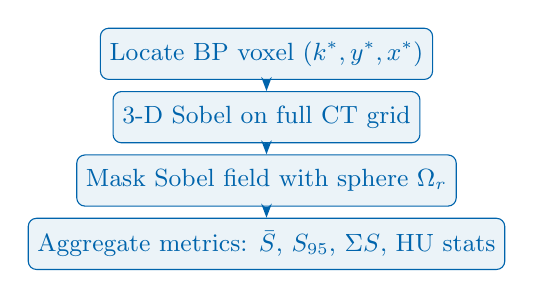
\begin{tikzpicture}[
        box/.style={draw=tudelft, rounded corners=3pt,
                    minimum width=3.0cm, minimum height=0.65cm,
                    font=\small, text=tudelft, fill=tudelft!8},
        arr/.style={-{Stealth[length=5pt]}, thick, tudelft},
        scale=0.95
      ]
        \node[box] (bp)   {Locate BP voxel $(k^*,y^*,x^*)$};
        \node[box, below=4pt of bp] (sob)
          {3-D Sobel on full CT grid};
        \node[box, below=4pt of sob] (sph)
          {Mask Sobel field with sphere $\Omega_r$};
        \node[box, below=4pt of sph] (met)
          {Aggregate metrics: $\bar{S}$, $S_{95}$, $\Sigma S$, HU stats};
        \draw[arr] (bp) -- (sob);
        \draw[arr] (sob) -- (sph);
        \draw[arr] (sph) -- (met);
      \end{tikzpicture}
      \end{center}

      \vspace{4pt}
      \begin{center}
      {\small
      \begin{tabular}{lcc}
        \toprule
        & \textbf{BP-range} & \textbf{Sphere} \\
        \midrule
        Geometry   & variable & fixed \\
        Length     & $\propto E$ & $r = \text{const}$ \\
        Hyperpar.  & $\alpha$, $\beta$ fractions & $r$ [mm] \\
        Lateral    & full beam & within $r$ \\
        \bottomrule
      \end{tabular}
      }
      \end{center}
    \end{column}
  \end{columns}
\end{frame}

% ════════════════════════════════════════════════════════════
\section{New Metrics: Pflugfelder HI \& WEPL}
% ════════════════════════════════════════════════════════════

\begin{frame}{New Metrics: Pflugfelder HI \& WEPL}
  \begin{columns}[T]
    \begin{column}{0.52\textwidth}
      \textbf{Water-Equivalent Path Length (WEPL)}\\
      For each lateral ray $(y, x)$ through the CT:
      \begin{equation*}
        \text{WEPL}(y,x)
        = \Delta z \sum_{k=0}^{k^*}
          \text{RSP}(k, y, x)
      \end{equation*}
      $\text{RSP}$ = relative stopping power (HU $\to$ RSP
      via Schneider calibration);
      $k^*$ = BP slice index.

      \vspace{2pt}
      WEPL map $\in \mathbb{R}^{H \times W}$: water-equivalent
      range to BP per lateral ray.

      \vspace{4pt}
      \textbf{Output scalars per beamlet:}
      \begin{itemize}\setlength{\itemsep}{0pt}
        \item \texttt{wepl\_mean} $= \mu(\text{WEPL})$ [mm]
        \item \texttt{wepl\_std} $= \sigma(\text{WEPL})$ [mm]
        \item \texttt{pflugfelder\_hi} $= \text{HI}$
      \end{itemize}
    \end{column}
    \begin{column}{0.44\textwidth}
      \textbf{Heterogeneity Index (HI)}~\cite{pflugfelder2007}:
      \begin{equation*}
        \text{HI} = \frac{\sigma(\text{WEPL})}{\mu(\text{WEPL})}
      \end{equation*}
      Computed over the flux footprint (10\,\% threshold).

      \vspace{4pt}
      \textbf{Interpretation}:
      \begin{itemize}\setlength{\itemsep}{1pt}
        \item HI $\approx 0$: homogeneous path (pure water).
        \item HI $\gg 0$: large lateral stopping-power
              variation $\to$ range uncertainty.
      \end{itemize}

      \vspace{4pt}
      \textbf{Motivation}: operates in dose space (mm of
      water) rather than image space (HU) — complementary
      to Sobel and HU metrics.

      \vspace{4pt}
      {\footnotesize Pflugfelder, Wilkens, Oelfke,
      \textit{Phys.~Med.~Biol.} 53(6):1689, 2007.}
    \end{column}
  \end{columns}
\end{frame}

\begin{frame}{HU $\rightarrow$ Material Composition $\rightarrow$ Density}
  \vspace{-2pt}
  {\footnotesize
  Schneider calibration is applied voxel-wise to map CT numbers to
  material class and physical density, which then drives the downstream
  RSP/WEPL calculations. The two examples below illustrate the same
  conversion pipeline for a high-energy and a low-energy beamlet.}

  \vspace{2pt}
  \begin{columns}[T]
    \begin{column}{0.49\textwidth}
      \begin{center}
        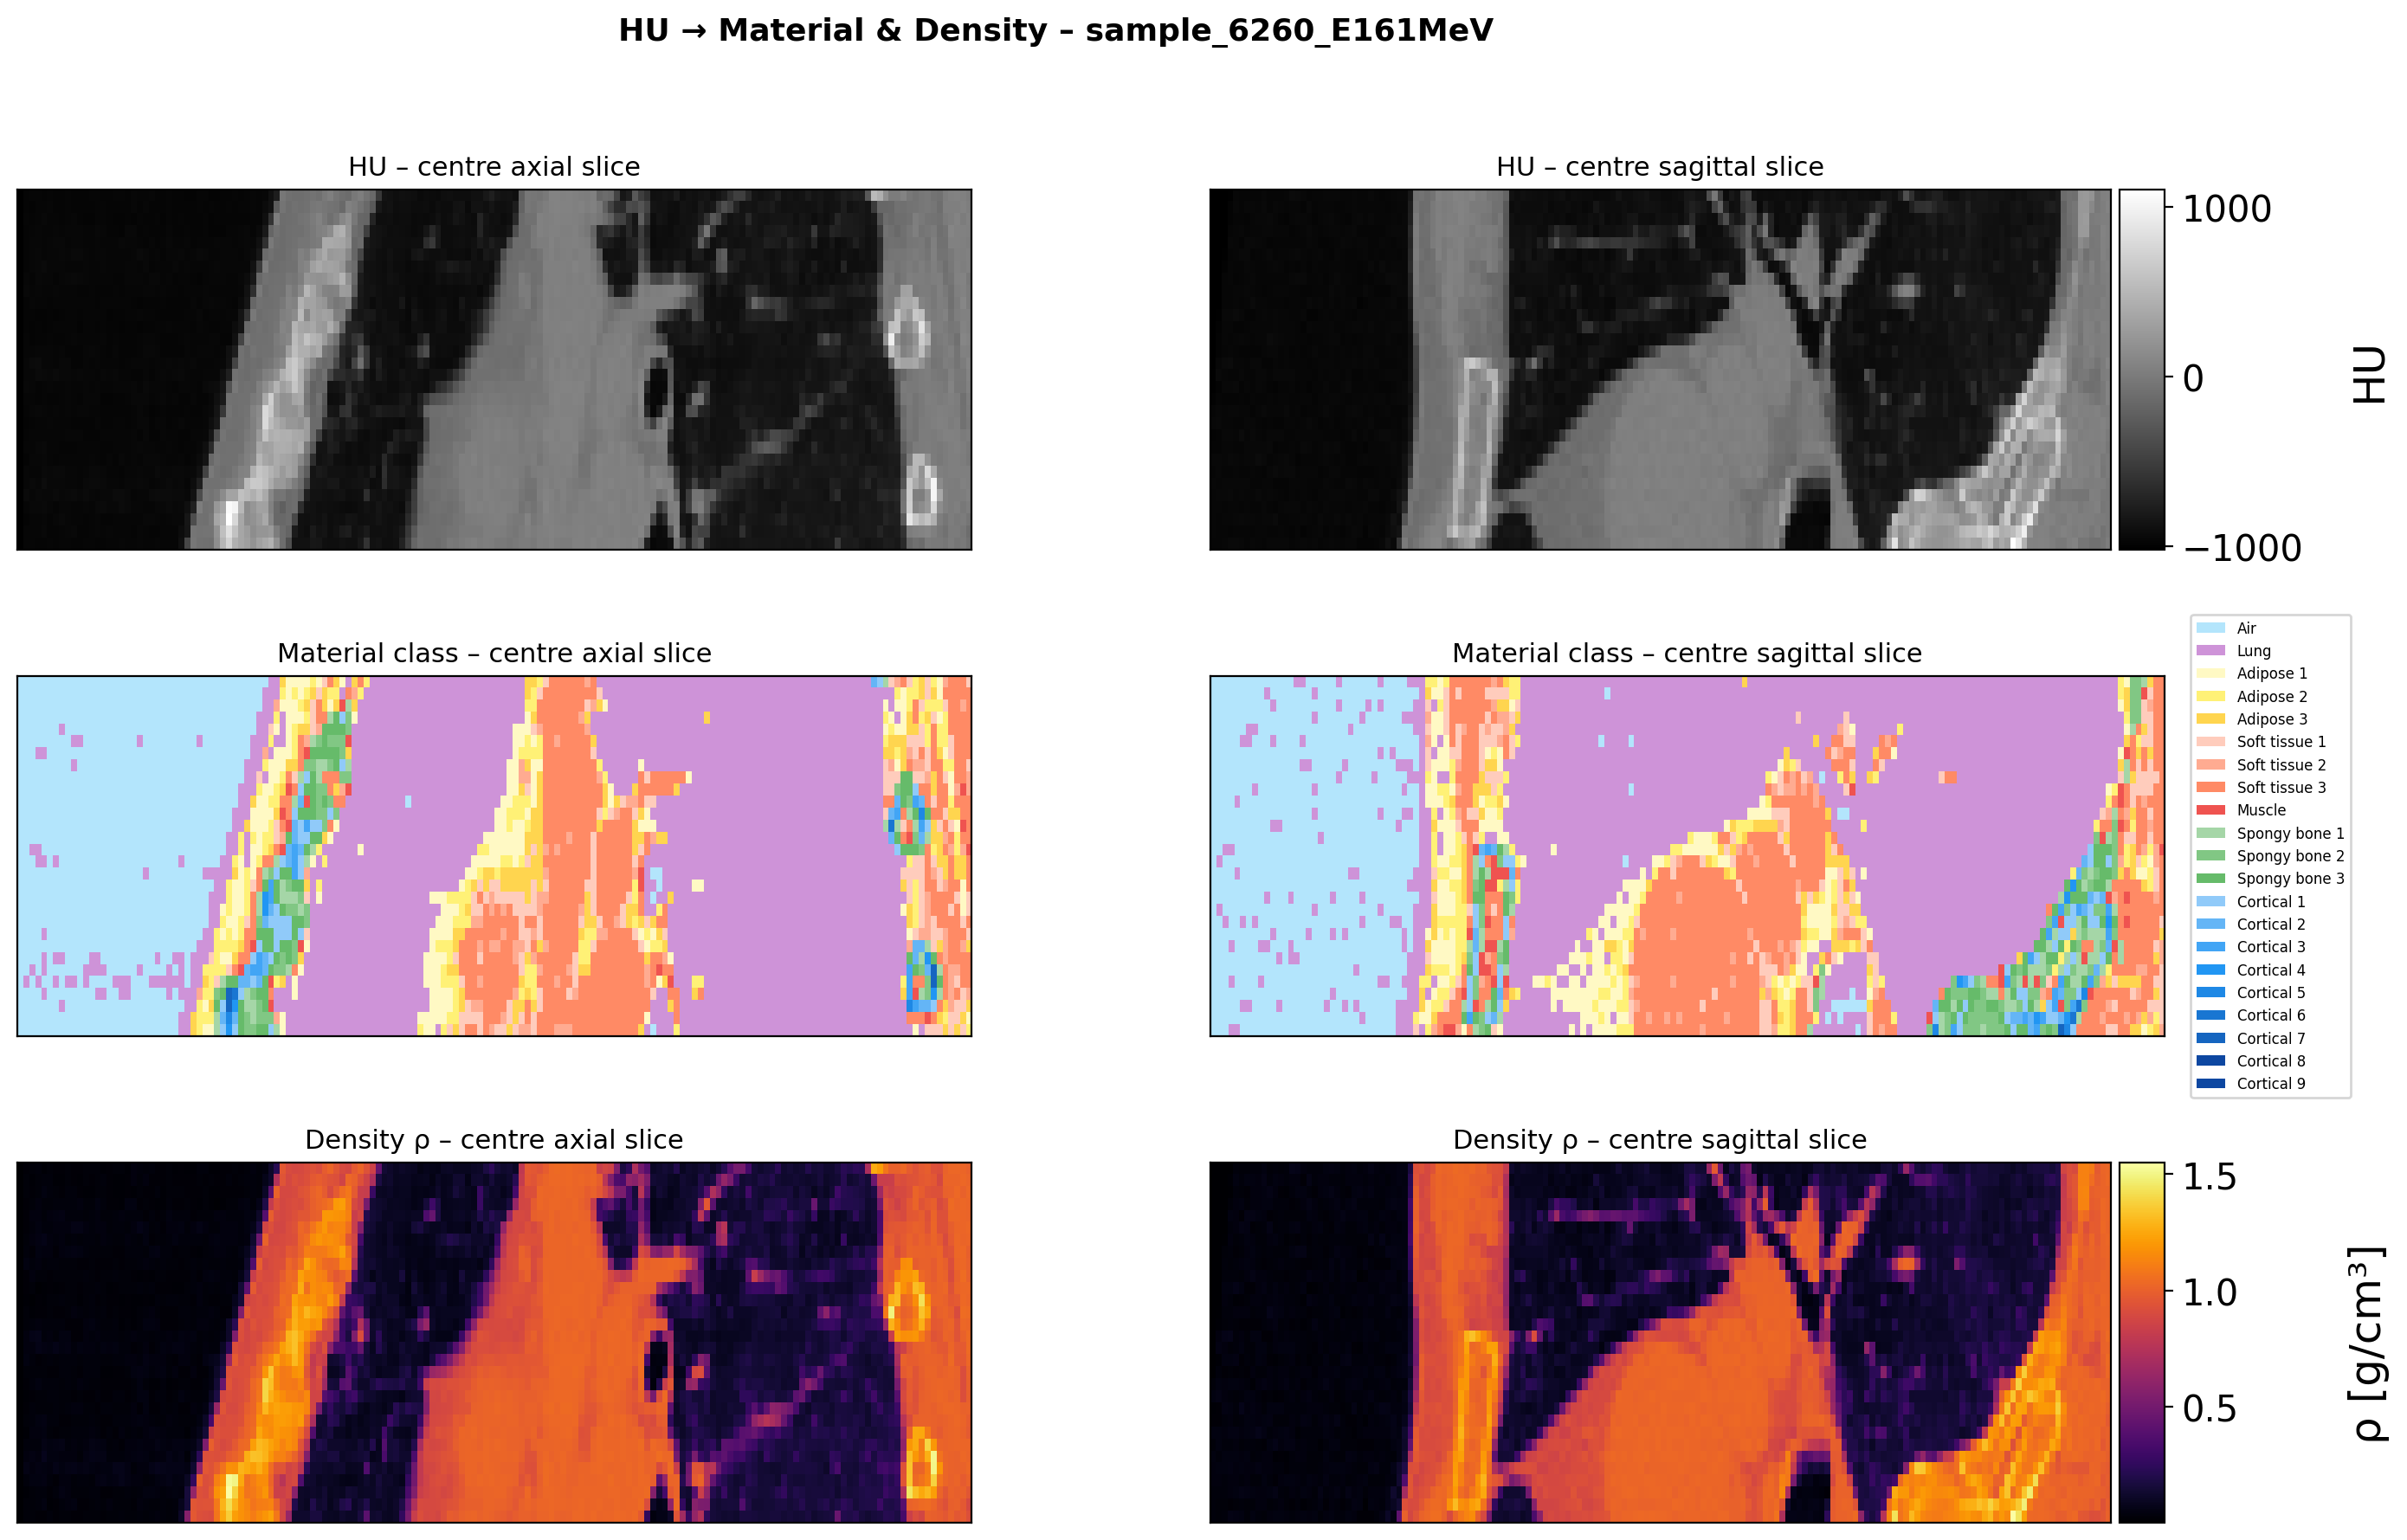
\includegraphics[width=\textwidth,height=0.55\textheight,keepaspectratio]{sample_6260_E161MeV_hu_material_density.png}\\[2pt]
        {\scriptsize Example 1: sample 6260}
      \end{center}
    \end{column}
    \begin{column}{0.49\textwidth}
      \begin{center}
        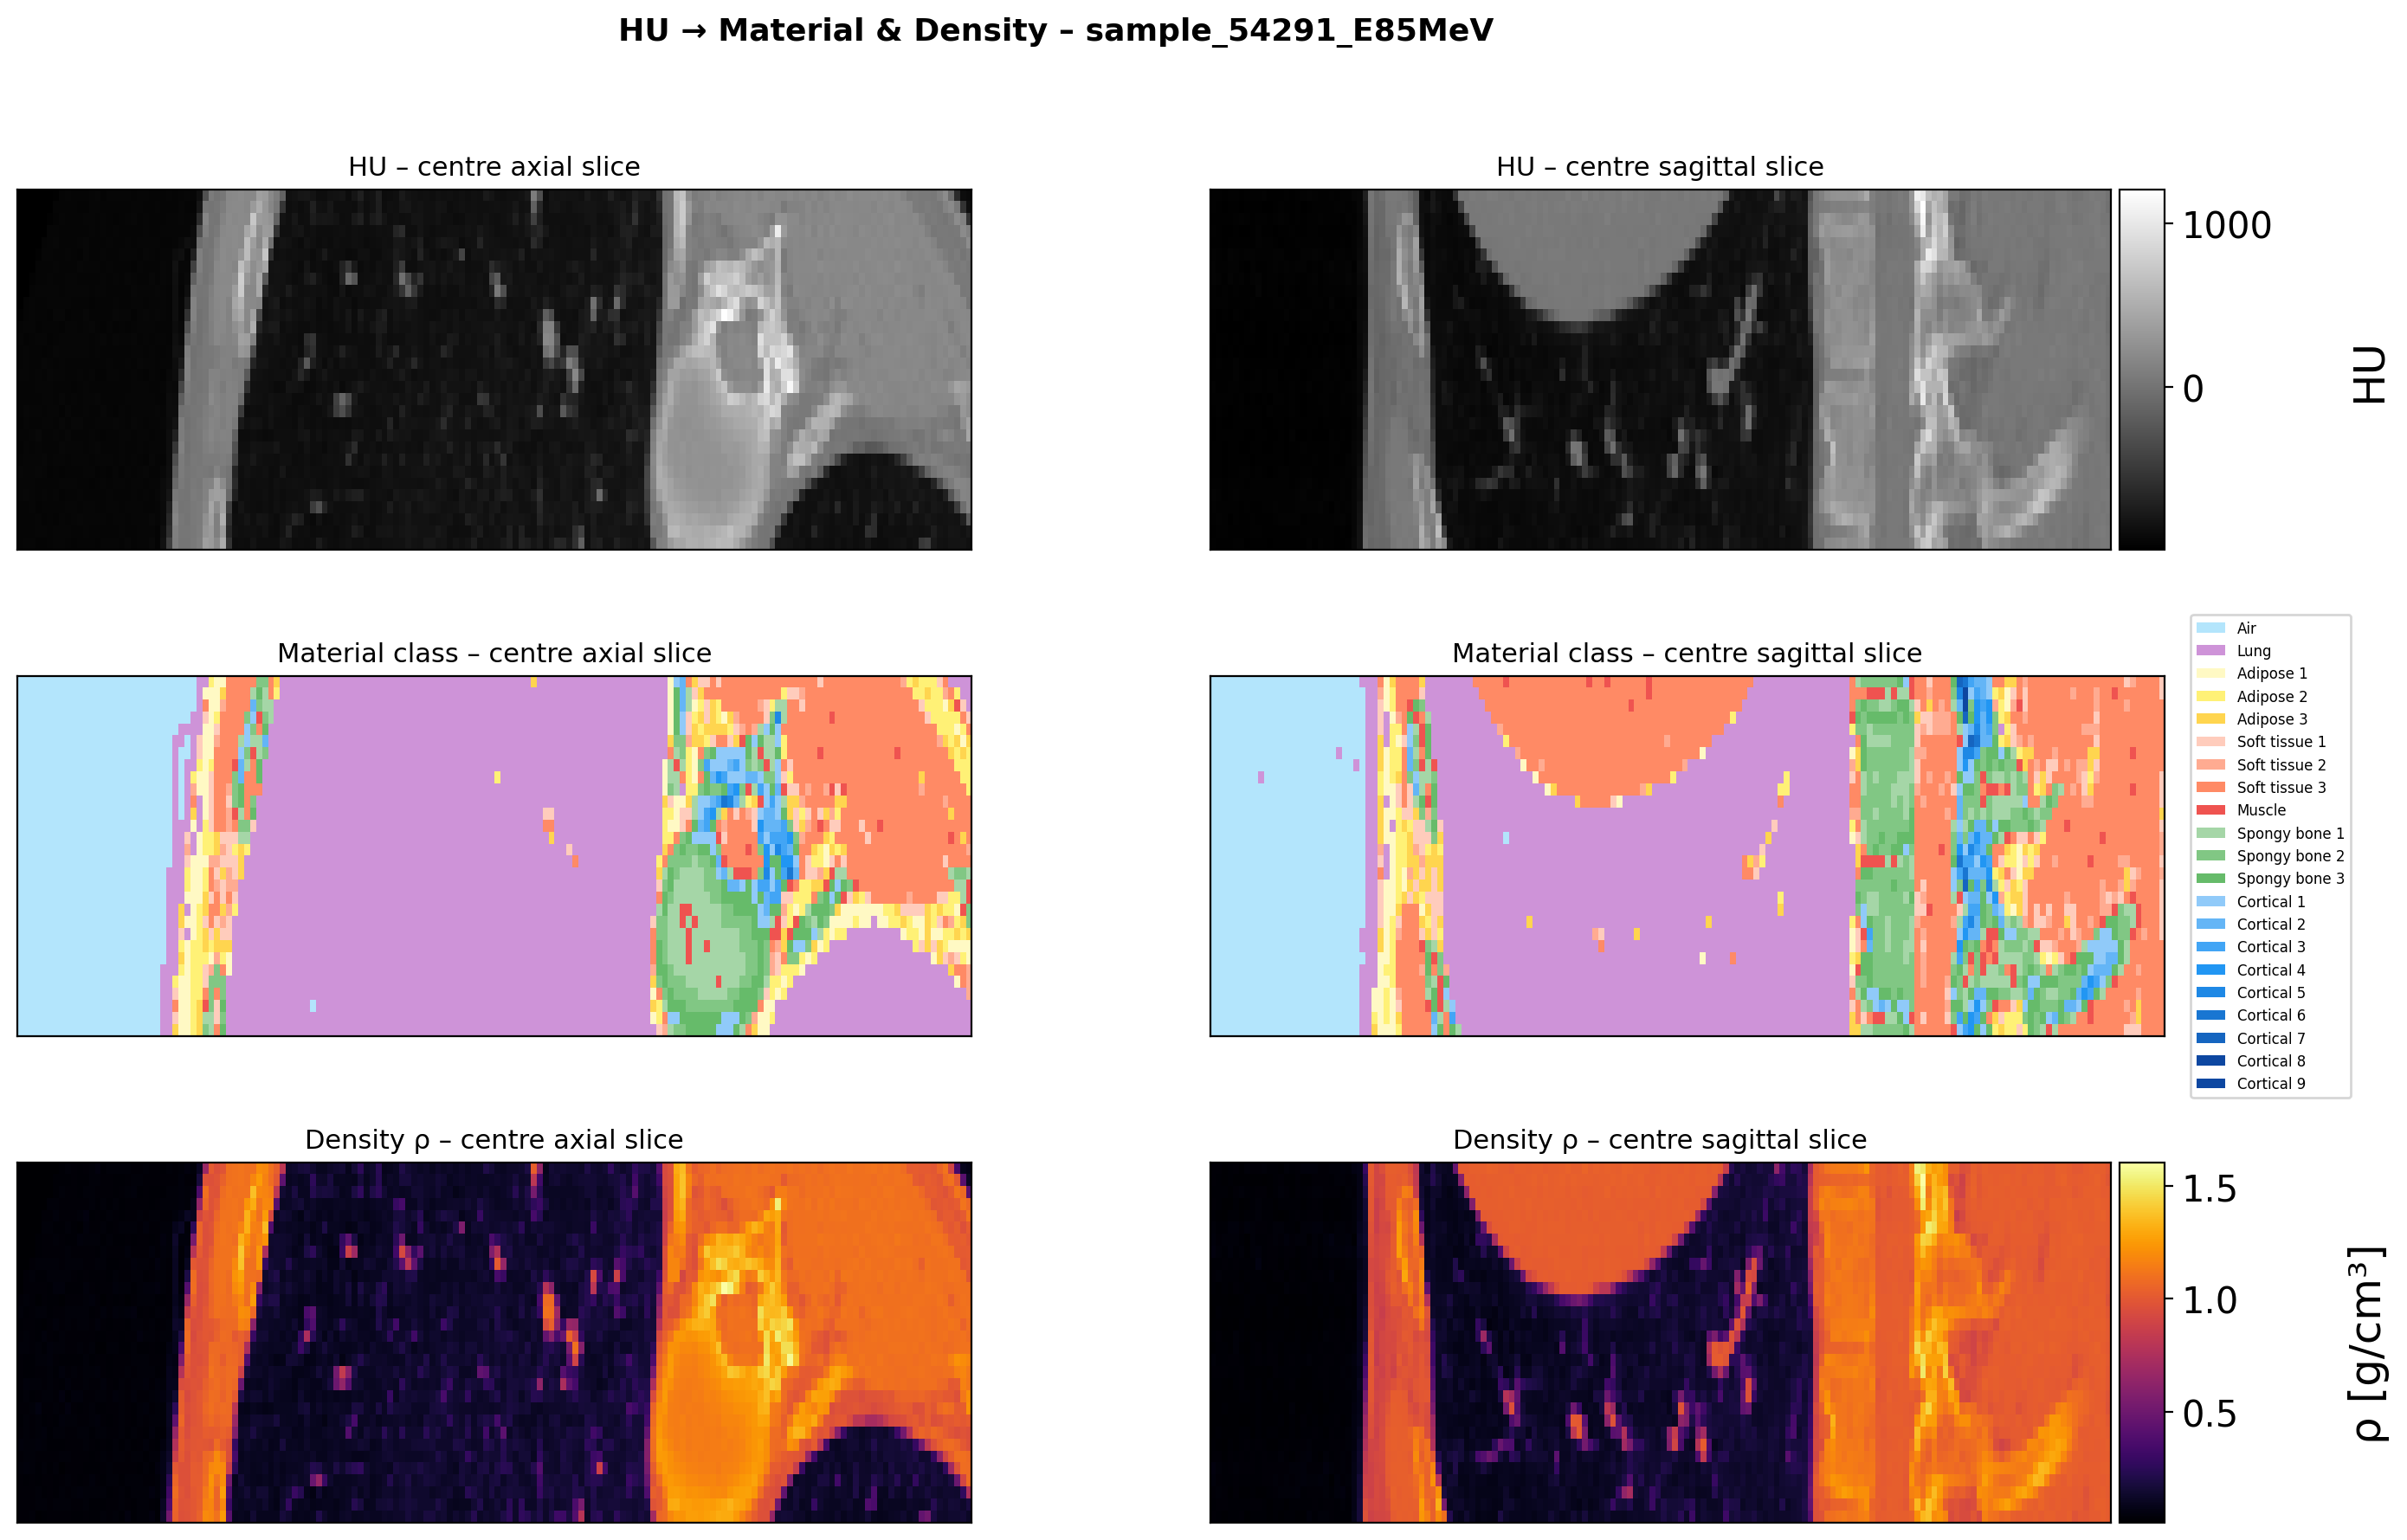
\includegraphics[width=\textwidth,height=0.55\textheight,keepaspectratio]{sample_54291_E85MeV_hu_material_density.png}\\[2pt]
        {\scriptsize Example 2: sample 54291}
      \end{center}
    \end{column}
  \end{columns}
\end{frame}

% ════════════════════════════════════════════════════════════
\section{Results: Full Database}
% ════════════════════════════════════════════════════════════

\begin{frame}{Scale-Up Completed: Dataset \& Model Inference}
  \begin{columns}[T]
    \begin{column}{0.48\textwidth}
      \textbf{Dataset:}
      \begin{itemize}
        \item $n = 69\,295$ beamlets (full ADoTA training set)
        \item 853 skipped (zero flux or duplicate)
        \item Energy range: \SIrange{70}{250}{MeV}
        \item Grid: $160 \times 30 \times 30$ voxels,
              $2 \times 2 \times \SI{2}{mm}$
      \end{itemize}

      \vspace{6pt}
      \textbf{Model}: ADoTA v3 (DoTA\_v3\_grid\_search\_v11)\\
      Gamma: $2\%/\SI{2}{mm}$, 10\,\% lower dose cutoff

      \vspace{6pt}
      \textbf{GPR distribution (overall):}\\
      Mean $= 98.83\%$, $\sigma = 1.47\%$\\
      Range: $[57.22\%,\; 100.00\%]$
    \end{column}
    \begin{column}{0.48\textwidth}
      \textbf{Energy bin distribution:}
      \vspace{4pt}
      \begin{center}
        \begin{tabular}{crc}
          \toprule
          \textbf{Bin (MeV)} & \textbf{$n$} & \textbf{GPR (\%)} \\
          \midrule
          70--100  & 16\,163 & $98.46 \pm 1.85$ \\
          100--130 & 15\,869 & $98.76 \pm 1.58$ \\
          130--160 & 16\,995 & $98.91 \pm 1.41$ \\
          160--190 & 13\,881 & $99.21 \pm 0.96$ \\
          190--220 &  3\,231 & $99.16 \pm 0.63$ \\
          220--250 &  3\,156 & $98.63 \pm 0.76$ \\
          \bottomrule
        \end{tabular}
      \end{center}
      {\small \textbf{Takeaway}: the 18$\times$ larger run preserves the
      same broad pattern as last week: lower-energy beamlets show larger
      GPR variance and therefore more room for heterogeneity effects to appear.}
    \end{column}
  \end{columns}
\end{frame}

\begin{frame}{Overall Correlation Ranking ($n = 69\,295$, $r = \SI{15}{mm}$)}
  \begin{columns}[T]
    \begin{column}{0.44\textwidth}
      \vspace{-4pt}
      
\includegraphics[width=\textwidth]{correlation_ranking.png}
    \end{column}
    \begin{column}{0.54\textwidth}
      \vspace{-4pt}
      {\scriptsize
      \setlength{\tabcolsep}{4pt}
      \renewcommand{\arraystretch}{0.95}
      \begin{tabular}{lrr}
        \toprule
        \textbf{Metric} & \textbf{Spearman} & \textbf{Pearson} \\
        \midrule
        sum\_sobel\_bp           & $-0.385$ & $-0.352$ \\
        hu\_change\_per\_region  & $-0.339$ & $-0.286$ \\
        p95\_sobel\_bp           & $-0.322$ & $-0.260$ \\
        $\sigma_{\text{HU}}$ at BP & $-0.310$ & $-0.239$ \\
        lateral\_hu\_var\_bp     & $-0.310$ & $-0.267$ \\
        hu\_change\_per\_mm      & $-0.297$ & $-0.183$ \\
        bp\_range\_mm            & $-0.293$ & $-0.047$ \\
        max\_hu\_jump            & $-0.291$ & $-0.229$ \\
        max\_hu\_gradient        & $-0.291$ & $-0.164$ \\
        total\_hu\_change        & $-0.285$ & $-0.059$ \\
        $n_{\text{regions}}$     & $-0.268$ & $-0.048$ \\
        hetero\_fraction         & $-0.268$ & $-0.143$ \\
        \textbf{pflugfelder\_hi} & $\mathbf{-0.242}$ & $\mathbf{-0.127}$ \\
        interface\_bp\_dist.     & $+0.141$ & $+0.065$ \\
        \bottomrule
      \end{tabular}
      }

      \vspace{2pt}
      {\scriptsize All $p \approx 0$.  \textbf{Bold}: new metric.
      Spearman $\gg$ Pearson $\Rightarrow$ monotonic but non-linear
      relationships.\\
      \textbf{Takeaway}: Sobel-based heterogeneity remains the strongest
      family of predictors after scale-up. The change from
      $S_{95,\text{BP}}$ to $\Sigma S_{\text{BP}}$ reflects the new
      sphere geometry, not a loss of signal.}
    \end{column}
  \end{columns}
\end{frame}

\begin{frame}{Best Predictor: Sum Sobel in BP Sphere}
  \vspace{-4pt}
  \begin{center}
    \includegraphics[height=0.64\textheight]{sum_sobel_bp_vs_gpr.png}
  \end{center}
  \vspace{-6pt}
  {\small $\Sigma S_{\text{BP}}$ achieves Spearman $\rho = -0.385$
  (Pearson $r = -0.352$, $p \approx 0$, $n = 69\,295$).
  Practical interpretation: beamlets with stronger local edge content near
  the Bragg peak tend to have worse GPR. The effect size is essentially
  unchanged relative to last week's smaller experiment.}
\end{frame}

% ════════════════════════════════════════════════════════════
\section{Energy-Stratified Analysis}
% ════════════════════════════════════════════════════════════

\begin{frame}{Why Check Energy Stratification?}
  \textbf{Observation} (confirmed at full scale):
  lower-energy bins show greater GPR variance ($\sigma \approx 1.85\%$
  at 70--100\,MeV vs.\ $0.63\%$ at 190--220\,MeV).

  \vspace{6pt}
  \textbf{Question}: are heterogeneity--GPR correlations genuine,
  or are they confounded by beam energy?

  \vspace{8pt}
  \textbf{Three complementary analyses}:
  \begin{enumerate}
    \item \textbf{Binned correlations}: Spearman $\rho$ within each
          \SI{30}{MeV} energy bin independently.
    \item \textbf{Energy-coloured scatter plots}: visualise
          metric vs.\ GPR coloured by energy.
    \item \textbf{Partial correlations}: partial Spearman
          controlling for energy,
          \begin{equation*}
            \rho_{XY \cdot Z} =
            \frac{\rho_{XY} - \rho_{XZ}\,\rho_{YZ}}
                 {\sqrt{(1-\rho_{XZ}^2)(1-\rho_{YZ}^2)}}
          \end{equation*}
          where $X$ = metric, $Y$ = GPR, $Z$ = energy.
  \end{enumerate}
\end{frame}

\begin{frame}{Spearman Correlation by Energy Bin}
  \begin{center}
    
\includegraphics[height=0.70\textheight]{spearman_heatmap_by_energy.png}
  \end{center}
  \vspace{-8pt}
  {\footnotesize \textbf{Takeaway}: correlations are strongest at low energies.
  70--100\,MeV: $|\rho| > 0.60$ for HU-change metrics and $> 0.48$
  for Sobel metrics. Above \SI{160}{MeV}, correlations largely vanish.
  This suggests the heterogeneity signal matters most in the clinically
  harder low-energy regime.}
\end{frame}

\begin{frame}[shrink=3]{Energy-Coloured Scatter: Sum Sobel at BP}
  \begin{center}
    \includegraphics[height=0.74\textheight]{sum_sobel_bp_vs_gpr_energy_coloured.png}
  \end{center}
  \vspace{-6pt}
  {\small Low-energy beamlets (dark) cluster in the high-$\Sigma S$ /
  low-GPR region; high-energy beamlets (bright) populate the
  compressed-metric / high-GPR region.  The energy gradient is
  visible but does \emph{not} drive the correlation (see partial
  analysis).}
\end{frame}

\begin{frame}{Partial Correlations Controlling for Energy}
  \begin{columns}[T]
    \begin{column}{0.52\textwidth}
      \vspace{-4pt}
      
\includegraphics[width=\textwidth]{partial_vs_raw_correlation.png}
    \end{column}
    \begin{column}{0.46\textwidth}
      \vspace{2pt}
      {\small
      \begin{tabular}{lrr}
        \toprule
        \textbf{Metric} & \textbf{Raw} & \textbf{Partial} \\
        \midrule
        sum\_sobel\_bp        & $-0.385$ & $-0.383$ \\
        hu\_change/region     & $-0.339$ & $-0.341$ \\
        $\sigma_{\text{HU,BP}}$ & $-0.310$ & $-0.334$ \\
        p95\_sobel\_bp        & $-0.322$ & $-0.322$ \\
        $n_{\text{regions}}$  & $-0.268$ & $-0.309$ \\
        max\_hu\_gradient     & $-0.291$ & $-0.309$ \\
        \bottomrule
      \end{tabular}
      }

      \vspace{6pt}
      {\small Raw and partial correlations differ by $|\Delta| < 0.04$:
      the heterogeneity--GPR association is \textbf{not confounded by
      energy}. Energy changes the variance structure, but it does not explain
      away the metric--GPR relationship.}
    \end{column}
  \end{columns}
\end{frame}

% ════════════════════════════════════════════════════════════
\section{Case Studies}
% ════════════════════════════════════════════════════════════

{
\setbeamertemplate{footline}{}
\begin{frame}[plain]{Worst-GPR Beamlet: \texttt{1f279484},
  \SI{120.67}{MeV}, GPR\,=\,57.22\,\%}
  \vspace{-4pt}
  \begin{columns}[T]
    \begin{column}{0.50\textwidth}
      \begin{center}
        \includegraphics[width=\textwidth,height=0.82\textheight,keepaspectratio]%
          {92669732-f19e-45e3-bf84-844f57e04133_ct_seg.png}\\
        {\scriptsize CT \& tissue segmentation along the beam}
      \end{center}
    \end{column}
    \begin{column}{0.50\textwidth}
      \begin{center}
        \includegraphics[width=\textwidth,height=0.82\textheight,keepaspectratio]%
          {1f279484_dose.png}\\
        {\scriptsize Dose: ground truth vs.\ ADoTA prediction}
      \end{center}
    \end{column}
  \end{columns}
\end{frame}
}

{
\setbeamertemplate{footline}{}
\begin{frame}[plain]{Best-GPR Beamlet: \texttt{ffa7d740},
  \SI{93.87}{MeV}, GPR\,=\,100.00\,\%}
  \vspace{-4pt}
  \begin{columns}[T]
    \begin{column}{0.50\textwidth}
      \begin{center}
        \includegraphics[width=\textwidth,height=0.82\textheight,keepaspectratio]%
          {ffa7d740-9119-4f00-ad47-e818e0584544_ct_seg.png}\\
        {\scriptsize CT \& tissue segmentation along the beam}
      \end{center}
    \end{column}
    \begin{column}{0.50\textwidth}
      \begin{center}
        \includegraphics[width=\textwidth,height=0.82\textheight,keepaspectratio]%
          {ffa7d740_dose.png}\\
        {\scriptsize Dose: ground truth vs.\ ADoTA prediction}
      \end{center}
    \end{column}
  \end{columns}
\end{frame}
}

% ════════════════════════════════════════════════════════════
\section{Sphere Radius Sensitivity}
% ════════════════════════════════════════════════════════════

\begin{frame}{$\Sigma S_{\text{BP}}$ vs.\ GPR: $r=\SI{15}{mm}$ vs $r=\SI{5}{mm}$}
  \vspace{-6pt}
  \begin{columns}[T]
    \begin{column}{0.50\textwidth}
      \begin{center}
        \includegraphics[width=\textwidth,height=0.56\textheight,keepaspectratio]%
          {sum_sobel_bp_vs_gpr_r15.png}\\[1pt]
        {\footnotesize $r = \SI{15}{mm}$ \;
        Spearman $\rho = -0.385$, Pearson $r = -0.352$}
      \end{center}
    \end{column}
    \begin{column}{0.50\textwidth}
      \begin{center}
        \includegraphics[width=\textwidth,height=0.56\textheight,keepaspectratio]%
          {sum_sobel_bp_vs_gpr_r5.png}\\[1pt]
        {\footnotesize $r = \SI{5}{mm}$ \;
        Spearman $\rho = -0.295$, Pearson $r = -0.272$}
      \end{center}
    \end{column}
  \end{columns}

  \vspace{2pt}
  {\footnotesize \textbf{Why this matters}: at $r = \SI{5}{mm}$ the sphere
  collapses to only $\sim$65 voxels and the dynamic range of
  $\Sigma S_{\text{BP}}$ shrinks; the scatter compresses against the
  left-hand axis $\Rightarrow$ a clear loss of monotonic separation against
  GPR ($|\rho|$ drops by $23\%$ relative). The wider \SI{15}{mm} sphere
  captures enough surrounding edge structure for $\Sigma S_{\text{BP}}$
  to remain the strongest single predictor.
  \textbf{This motivates $r = \SI{15}{mm}$ as the working default.}}
\end{frame}

\begin{frame}[shrink=5]{Sphere Radius Comparison: \SI{15}{mm} vs \SI{5}{mm}}
  \begin{columns}[T]
    \begin{column}{0.54\textwidth}
      \vspace{-2pt}
      {\small
      \begin{tabular}{lrrr}
        \toprule
        \textbf{Metric} & $\rho_s^{15\text{mm}}$ & $\rho_s^{5\text{mm}}$ & $\Delta|\rho|$ \\
        \midrule
        \textbf{sum\_sobel\_bp}     & $\mathbf{-0.385}$ & $-0.295$ & $\mathbf{+0.090}$ \\
        \textbf{p95\_sobel\_bp}     & $\mathbf{-0.322}$ & $-0.292$ & $\mathbf{+0.030}$ \\
        mean\_sobel\_axial          & $-0.209$ & $-0.202$ & $+0.007$ \\
        \midrule
        hu\_change\_per\_region     & $-0.339$ & $-0.339$ & $0.000$ \\
        $\sigma_{\text{HU}}$ at BP  & $-0.310$ & $-0.310$ & $0.000$ \\
        lateral\_hu\_var\_bp        & $-0.310$ & $-0.310$ & $0.000$ \\
        hu\_change\_per\_mm         & $-0.297$ & $-0.297$ & $0.000$ \\
        max\_hu\_jump               & $-0.291$ & $-0.291$ & $0.000$ \\
        max\_hu\_gradient           & $-0.291$ & $-0.291$ & $0.000$ \\
        total\_hu\_change           & $-0.285$ & $-0.285$ & $0.000$ \\
        $n_{\text{regions}}$        & $-0.268$ & $-0.268$ & $0.000$ \\
        hetero\_fraction            & $-0.268$ & $-0.268$ & $0.000$ \\
        pflugfelder\_hi             & $-0.242$ & $-0.242$ & $0.000$ \\
        wepl\_std                   & $-0.231$ & $-0.231$ & $0.000$ \\
        interface\_bp\_dist.        & $+0.141$ & $+0.141$ & $0.000$ \\
        \bottomrule
      \end{tabular}
      }
    \end{column}
    \begin{column}{0.44\textwidth}
      \textbf{Key observation}: \emph{only the Sobel metrics depend
      on sphere radius}.  All HU and WEPL/Pflugfelder metrics are
      radius-invariant.

      \vspace{4pt}
      \textbf{Why?} The HU metrics
      (\texttt{hu\_change\_per\_region}, $\sigma_{\text{HU,BP}}$,
      $\Delta H_{\max}$, …) are computed on the
      \emph{flux-weighted axial HU profile} over $[z_{\min}, z_{\max}]$
      and on the \emph{lateral BP slice}.  WEPL is computed over the
      full lateral footprint up to $k^*$.  Only the
      Sobel-family aggregation is bounded by the sphere $\Omega_r$.

      \vspace{4pt}
      \textbf{Effect on Sobel metrics}:
      \begin{itemize}\setlength{\itemsep}{0pt}
        \item $\Sigma S_{\text{BP}}$: $|\rho_s|$ drops from
              $0.385 \to 0.295$ ($-23\%$ relative)
        \item $S_{95,\text{BP}}$: $0.322 \to 0.292$ ($-9\%$)
        \item $\bar{S}_{\text{axial}}$: essentially unchanged
      \end{itemize}

      \vspace{4pt}
      \textbf{Completed result}: the $r = \SI{5}{mm}$ experiment confirms
      the same overall ranking, but with weaker Sobel-family performance.\\[4pt]

      \textbf{Recommendation}: adopt \textbf{$r = \SI{15}{mm}$} as
      the default. It strictly dominates $r = \SI{5}{mm}$ on
      Sobel-family metrics and is identical for everything else.
      Energy-stratified and partial-correlation patterns
      reproduce the 15 mm results (not shown for brevity).
    \end{column}
  \end{columns}
\end{frame}

% ════════════════════════════════════════════════════════════
\section{Discussion \& Key Findings}
% ════════════════════════════════════════════════════════════

\begin{frame}{Key Findings}
  \begin{enumerate}
    \item \textbf{Scale confirmed}: findings from last week
          ($n = 3\,950$) fully replicated at $n = 69\,295$ ($18\times$
          larger). Sobel-based metrics remain the strongest
          single predictors of GPR degradation.

    \vspace{4pt}
    \item \textbf{Sphere method}: switching from BP-range to sphere
          changes the leading metric from $S_{95,\text{BP}}$ to
          $\Sigma S_{\text{BP}}$ (sum vs.\ percentile), but both
          reach $|\rho_s| \approx 0.38$--$0.39$ — essentially
          equivalent predictive power.

    \vspace{4pt}
    \item \textbf{Energy-stratification at scale}:
          correlations strongest at 70--100\,MeV ($|\rho_s| > 0.60$
          for HU-change metrics), weaken above \SI{160}{MeV}.
          Partial correlations confirm energy is \emph{not} a confounder
          ($|\Delta\rho| < 0.04$).

    \vspace{4pt}
    \item \textbf{Pflugfelder HI}: achieves Spearman $\rho = -0.242$
          (rank \#13 of 17).  Clinically interpretable (water-equivalent
          units) but weaker than Sobel metrics.
          WEPL std ($\rho = -0.231$) is similar.

    \vspace{4pt}
    \item \textbf{Radius sensitivity}: only Sobel metrics depend on
          the sphere radius. $\Sigma S_{\text{BP}}$ drops from
          $\rho_s = -0.385$ at $r = \SI{15}{mm}$ to $-0.295$ at
          $r = \SI{5}{mm}$ (a $23\%$ relative loss); HU and
          WEPL/Pflugfelder metrics are unchanged.
          \textbf{Recommendation}: use $r = \SI{15}{mm}$ as the default
          for the next iteration.
  \end{enumerate}
\end{frame}

\begin{frame}{Discussion Points for Today}
  \begin{enumerate}
    \item \textbf{Method choice}: proceed with the sphere method and
          standardise on $r = \SI{15}{mm}$?

    \vspace{6pt}
    \item \textbf{Priority for next week}: should the focus be on
          a stronger engineered metric (ISI / composite score) or on
          the VLM proof-of-concept?

    \vspace{6pt}
    \item \textbf{Validation direction}: is the next most useful step
          a held-out evaluation, or a clinical interpretation of the
          worst-performing low-energy beamlets?
  \end{enumerate}
\end{frame}

% ════════════════════════════════════════════════════════════
\section{Next Steps}
% ════════════════════════════════════════════════════════════

\begin{frame}{Next Steps}
  \begin{enumerate}
    \item \textbf{Interface Severity Index (ISI)}:
          per-class interface-pair severity matrix
          ($W_{ab} = (\Delta\mathrm{RSP})^2$) using the Schneider
          24-class decomposition, aggregated within the $r = \SI{15}{mm}$
          BP sphere. This is the most direct next engineered metric.

    \vspace{6pt}
    \item \textbf{Composite difficulty score}: combine top metrics
          ($\Sigma S_{\text{BP}}$, $\sigma_{\text{HU,BP}}$,
          $\Delta H / n_{\text{reg}}$) into a single ``difficulty index''
          via PCA or logistic regression on the full $n = 69\,295$
          dataset.

    \vspace{6pt}
    \item \textbf{VLM difficulty estimation}: implement Track~A
          (zero-shot) as a proof-of-concept and compare Spearman $\rho$
          against engineered metrics on a held-out subset.

    \vspace{6pt}
    \item \textbf{Worst-case deep-dive}: visualise and analyse the
          beamlets with GPR $< 90\%$ in the 70--100\,MeV bin to
          identify anatomical patterns driving failure.
  \end{enumerate}
\end{frame}

% ════════════════════════════════════════════════════════════
\begin{frame}[plain]
  \centering
  \vfill
  {\Large\bfseries\color{tudelft} Questions?}
  \vfill
\end{frame}

% ── References ──────────────────────────────────────────────
\begin{frame}{References}
  \small
  \begin{thebibliography}{9}
    \bibitem{pflugfelder2007}
    D.~Pflugfelder, J.~J.~Wilkens, U.~Oelfke,
    ``Worst case optimization: a method to account for uncertainties
    in the optimization of intensity modulated proton therapy,''
    \textit{Phys.~Med.~Biol.}, vol.~53, no.~6, pp.~1689--1700, 2007.\\
    \url{https://doi.org/10.1088/0031-9155/53/6/013}
  \end{thebibliography}
\end{frame}

\end{document}
